\documentclass[11pt, letterpaper]{article}

% Fonts and Encoding
\usepackage[utf8]{inputenc}
\usepackage[T1]{fontenc}
\usepackage{lmodern} % High-quality Latin Modern vector font

% Math and Symbols
\usepackage{amsmath, amssymb, amsthm, amsfonts, mathrsfs, mathtools}

% Layout and Geometry
\usepackage{geometry}
\geometry{letterpaper, margin=1in}
\setlength{\parindent}{0pt}
\setlength{\parskip}{0.6em}

% Formatting and Graphics
\usepackage{graphicx, xcolor, enumitem, booktabs, array, tabularx}

% TikZ for Illustrations
\usepackage{tikz}
\usetikzlibrary{arrows.meta, positioning, shapes.geometric, calc, backgrounds, matrix}

% Clickable Links and TOC
\usepackage{hyperref}
\hypersetup{
    colorlinks=true,
    linkcolor=blue,
    filecolor=magenta,      
    urlcolor=cyan,
    pdftitle={Advanced Mathematics: Bijective Functions},
}

% Theorem Environments
\newtheorem{theorem}{Theorem}[section]
\newtheorem{lemma}[theorem]{Lemma}
\newtheorem{proposition}[theorem]{Proposition}
\newtheorem{corollary}[theorem]{Corollary}
\theoremstyle{definition}
\newtheorem{definition}{Definition}[section]
\newtheorem{axiom}{Axiom}[section]
\newtheorem{example}{Example}[section]
\theoremstyle{remark}
\newtheorem{remark}{Remark}[section]

% Custom Commands (Enforced standard notation)
\newcommand{\R}{\mathbb{R}}
\newcommand{\N}{\mathbb{N}}
\newcommand{\Z}{\mathbb{Z}}
\newcommand{\Q}{\mathbb{Q}}
\newcommand{\E}{\mathbb{E}}
\newcommand{\Prob}{\mathbb{P}}
\newcommand{\F}{\mathcal{F}}

\title{\textbf{Advanced Mathematics: Bijective Functions}\\ \Large Foundations, Proofs, and Applications in Quantitative Modeling}
\author{Tashfeen Omran}
\date{November 12, 2026}

\begin{document}

\maketitle
\tableofcontents
\newpage

\section{Concept Checklist \& Question Mapping}
\label{sec:concept_checklist_start}

This problem set rigorously tests the theoretical concepts, logical structures, and applied modeling techniques detailed in the foundational text. 

\renewcommand{\arraystretch}{1.5}
\begin{tabularx}{\textwidth}{>{\bfseries}l X >{$\displaystyle}c<{$}}
\toprule
\textbf{ID} & \textbf{Concept / Proof Technique} & \text{\textbf{Problems}} \\
\midrule
C1 & Algebraic Bijections (Linear, Quadratic, Rational) & 1, 2, 3, 4, 5 \\
C2 & Modular Arithmetic \& Equivalence Classes ($\Z_n$) & 6, 7, 8 \\
C3 & Set-Theoretic Proofs (Images, Pre-images, Subsets) & 9, 10, 11, 12 \\
C4 & Function Composition \& Left/Right Inverses & 13, 14, 15, 16 \\
C5 & Combinatorics, Pigeonhole, \& Hall's Marriage & 17, 18, 19, 20 \\
C6 & Calculus-Based Bijections (Derivatives, IVT) & 21, 22, 23 \\
C7 & Infinite Sets \& Cantor-Schröder-Bernstein Theorem & 24, 25, 26 \\
C8 & Real-World Modeling: Normalizing Flows \& Copulas & 27, 28, 29 \\
C9 & Logical Fallacies \& Axiomatic Edge Cases & 30 \\
\bottomrule
\end{tabularx}

\newpage

\section{Problem Sets}

\textbf{Algebraic Bijections}
\begin{enumerate}[label=\textbf{\arabic*.}]
    \item Prove that the function $f : \R \to \R$ defined by $f(x) = 4x - 9$ is bijective.
    \item Determine whether the function $f : \Z \to \Z$ defined by $f(n) = 3n + 2$ is bijective. Prove your assertion.
    \item Prove that the rational function $f : \R \setminus \{3\} \to \R \setminus \{2\}$ defined by $f(x) = \frac{2x+1}{x-3}$ is bijective.
    \item Find a counterexample to disprove the claim: ``The function $f : \R \to \R$ defined by $f(x) = x^2 - 8x + 17$ is bijective.''
    \item Restrict the domain and codomain of $f(x) = x^2 - 8x + 17$ to construct a valid bijective function where the domain is of the form $[k, \infty)$. Prove it is bijective on this restricted space.
\end{enumerate}

\textbf{Modular Arithmetic}
\begin{enumerate}[label=\textbf{\arabic*.}, resume]
    \item Let $f : \Z_7 \to \Z_7$ be defined by $f([x]) = [5x + 2]$. Prove that $f$ is well-defined and bijective.
    \item Show that the function $f : \Z_8 \to \Z_8$ defined by $f([x]) = [4x + 1]$ is not a bijection.
    \item Let $p$ be a prime number. Prove that $f : \Z_p \to \Z_p$ defined by $f([x]) = [ax + b]$ is a bijection if and only if $[a] \neq [0]$.
\end{enumerate}

\textbf{Set-Theoretic Proofs}
\begin{enumerate}[label=\textbf{\arabic*.}, resume]
    \item Let $f : A \to B$ be a function, and let $C, D \subseteq A$. Prove that $f(C \cup D) = f(C) \cup f(D)$.
    \item Let $f : A \to B$. Prove that $f$ is injective if and only if $f(C \cap D) = f(C) \cap f(D)$ for all subsets $C, D \subseteq A$.
    \item Let $f : A \to B$ be a function, and let $Y, Z \subseteq B$. Prove that $f^{-1}(Y \cup Z) = f^{-1}(Y) \cup f^{-1}(Z)$.
    \item Let $f : A \to B$ be a function, and let $Y, Z \subseteq B$. Prove that $f^{-1}(Y \cap Z) = f^{-1}(Y) \cap f^{-1}(Z)$.
\end{enumerate}

\textbf{Function Composition \& Inverses}
\begin{enumerate}[label=\textbf{\arabic*.}, resume]
    \item Let $f : A \to B$ and $g : B \to C$. Prove that if the composition $g \circ f$ is bijective, then $f$ is injective and $g$ is surjective.
    \item Provide a concrete counterexample showing that if $g \circ f$ is bijective, $f$ is not necessarily surjective.
    \item Prove that a function $f : A \to B$ is injective if and only if it has a left inverse (i.e., there exists $g : B \to A$ such that $g(f(x)) = x$ for all $x \in A$). Assume $A \neq \emptyset$.
    \item Prove that if a function $f : A \to B$ has a right inverse (i.e., there exists $h : B \to A$ such that $f(h(y)) = y$ for all $y \in B$), then $f$ is surjective.
\end{enumerate}

\textbf{Combinatorics, Pigeonhole, \& Hall's Marriage}
\begin{enumerate}[label=\textbf{\arabic*.}, resume]
    \item Let $A$ and $B$ be finite sets such that $|A| = |B| = n$. Prove that a function $f : A \to B$ is injective if and only if it is surjective.
    \item Use the Pigeonhole Principle to rigorously prove that no function $f : A \to B$ can be injective if $|A| = n + 1$ and $|B| = n$.
    \item Let $A = \{a, b, c\}$ and $B = \{1, 2, 3\}$. A relation defines the allowed mappings as $L(a) = \{1, 2\}$, $L(b) = \{1, 2\}$, and $L(c) = \{1, 2\}$. Use Hall's Marriage Condition to prove that no bijective function can be formed from these lists.
    \item Let $A = \{1, 2, 3, 4\}$ and $B = \{x, y, z, w\}$. A relation $R \subseteq A \times B$ is given by $R = \{(1, x), (1, y), (2, y), (2, z), (3, w), (4, w)\}$. Determine the domination number $\gamma(R)$ and justify your answer.
\end{enumerate}

\textbf{Calculus-Based Bijections}
\begin{enumerate}[label=\textbf{\arabic*.}, resume]
    \item Prove that the function $f : \R \to \R$ defined by $f(x) = x^3 + x$ is bijective.
    \item Prove that the function $f : \R \to \R$ defined by $f(x) = e^x + x$ is bijective.
    \item The function $f(x) = \sin(x)$ is not bijective on $\R \to \R$. Define the standard restricted domain and codomain that makes it bijective, and rigorously justify both injectivity and surjectivity on this restriction.
\end{enumerate}

\textbf{Infinite Sets \& Cantor-Schröder-Bernstein}
\begin{enumerate}[label=\textbf{\arabic*.}, resume]
    \item Construct an explicit injective function from $\N$ to $\Q$.
    \item Use the Cantor-Schröder-Bernstein Theorem to prove that the open interval $(0, 1)$ and the half-open interval $[0, 1)$ have the same cardinality.
    \item Prove Cantor's Theorem: There does not exist a surjective function from a set $A$ to its power set $\mathcal{P}(A)$.
\end{enumerate}

\textbf{Real-World Modeling: AI \& Quant Finance}
\begin{enumerate}[label=\textbf{\arabic*.}, resume]
    \item \textbf{Normalizing Flows:} Let $(\Omega, \F, \Prob)$ be a probability space. Let $Z \sim \mathcal{N}(0, 1)$ be a latent noise variable with PDF $p_Z(z) = \frac{1}{\sqrt{2\pi}} e^{-z^2/2}$. Let $f : \R \to (0, \infty)$ be the diffeomorphism $f(z) = e^z$. Define $X = f(Z)$. Use the pushforward measure (Change of Variables) to derive the exact probability density function $p_X(x)$.
    \item \textbf{Copulas:} Let $X$ be a strictly continuous random variable with a strictly increasing Cumulative Distribution Function (CDF) $F_X : \R \to (0, 1)$. Prove that the transformed random variable $U = F_X(X)$ follows a standard Uniform distribution on $(0, 1)$.
    \item \textbf{Jacobian Determinant:} Let $f : \R^2 \to \R^2$ be defined by $f(x, y) = (x + y, x - y)$. Prove that $f$ is a bijection and compute the determinant of its Jacobian matrix. Explain why a non-zero determinant is required for probability transformations.
\end{enumerate}

\textbf{Logical Fallacies}
\begin{enumerate}[label=\textbf{\arabic*.}, resume]
    \item Identify and rigorously explain the mathematical flaw in the following proof: \\
    \textit{Claim:} The function $f : \Z \to \Z$ defined by $f(n) = 4n$ is surjective. \\
    \textit{Proof:} Let $f(a) = f(b)$. Then $4a = 4b \implies a = b$. Thus, $f$ is injective. By Theorem 1.2 (Finiteness and Bijections), since the domain and codomain have the same cardinality ($|\Z| = |\Z|$), injectivity implies surjectivity. Therefore, $f$ is surjective. $\blacksquare$
\end{enumerate}

\newpage

\section{Detailed Solutions}

\begin{proof}[Solution to Problem 1]
We must prove $f(x) = 4x - 9$ is both injective and surjective on $\R$. \\
\textbf{Injectivity:} Let $a, b \in \R$ and assume $f(a) = f(b)$.
\[ 4a - 9 = 4b - 9 \implies 4a = 4b \implies a = b \]
Thus, $f$ is injective. \\
\textbf{Surjectivity:} Let $y \in \R$. We must find $x \in \R$ such that $f(x) = y$.
\[ 4x - 9 = y \implies 4x = y + 9 \implies x = \frac{y + 9}{4} \]
Since $y \in \R$, $x = \frac{y+9}{4} \in \R$. Furthermore, $f\left(\frac{y+9}{4}\right) = 4\left(\frac{y+9}{4}\right) - 9 = y + 9 - 9 = y$. Thus, $f$ is surjective. \\
Being both injective and surjective, $f$ is bijective.
\end{proof}

\begin{proof}[Solution to Problem 2]
We test $f(n) = 3n + 2$ for injectivity and surjectivity on $\Z$. \\
\textbf{Injectivity:} Let $a, b \in \Z$ and assume $f(a) = f(b)$.
\[ 3a + 2 = 3b + 2 \implies 3a = 3b \implies a = b \]
Thus, $f$ is injective. \\
\textbf{Surjectivity:} Let $y = 0 \in \Z$. We require $n \in \Z$ such that $3n + 2 = 0$.
\[ 3n = -2 \implies n = -\frac{2}{3} \]
Since $-\frac{2}{3} \notin \Z$, the element $0$ has no pre-image in $\Z$. Thus, $f$ is not surjective. \\
Consequently, $f$ is \textbf{not bijective}.
\end{proof}

\begin{proof}[Solution to Problem 3]
Let $f(x) = \frac{2x+1}{x-3}$ for $x \in \R \setminus \{3\}$. \\
\textbf{Injectivity:} Let $a, b \in \R \setminus \{3\}$ and assume $f(a) = f(b)$.
\[ \frac{2a+1}{a-3} = \frac{2b+1}{b-3} \]
Cross-multiplying yields:
\[ (2a+1)(b-3) = (2b+1)(a-3) \]
\[ 2ab - 6a + b - 3 = 2ab - 6b + a - 3 \]
Subtracting $2ab - 3$ from both sides:
\[ -6a + b = -6b + a \implies 7b = 7a \implies a = b \]
Thus, $f$ is injective. \\
\textbf{Surjectivity:} Let $y \in \R \setminus \{2\}$. We must find $x \in \R \setminus \{3\}$ such that $f(x) = y$.
\[ y = \frac{2x+1}{x-3} \implies y(x-3) = 2x+1 \implies yx - 3y = 2x + 1 \]
\[ yx - 2x = 3y + 1 \implies x(y-2) = 3y + 1 \implies x = \frac{3y+1}{y-2} \]
Since $y \neq 2$, $x$ is a well-defined real number. We must verify $x \neq 3$. Suppose for contradiction $x = 3$. Then $3 = \frac{3y+1}{y-2} \implies 3y - 6 = 3y + 1 \implies -6 = 1$, a contradiction. Thus $x \in \R \setminus \{3\}$. $f$ is surjective, and therefore bijective.
\end{proof}

\begin{proof}[Solution to Problem 4]
We complete the square for $f(x) = x^2 - 8x + 17$:
\[ f(x) = (x^2 - 8x + 16) + 1 = (x - 4)^2 + 1 \]
\textbf{Not Injective:} Let $x_1 = 3$ and $x_2 = 5$. $f(3) = (3-4)^2 + 1 = 2$. $f(5) = (5-4)^2 + 1 = 2$. Since $f(3) = f(5)$ but $3 \neq 5$, $f$ is not injective. \\
\textbf{Not Surjective:} For any $x \in \R$, $(x-4)^2 \ge 0$, so $f(x) \ge 1$. Let $y = 0 \in \R$. There is no $x \in \R$ such that $f(x) = 0$. Thus, $f$ is not surjective.
\end{proof}

\begin{proof}[Solution to Problem 5]
From Problem 4, $f(x) = (x-4)^2 + 1$. The vertex of this parabola is at $x = 4$. To make the function strictly increasing (and thus injective), we restrict the domain to $[4, \infty)$. The minimum value is $f(4) = 1$, so we restrict the codomain to $[1, \infty)$. \\
Let $f : [4, \infty) \to [1, \infty)$ be defined by $f(x) = (x-4)^2 + 1$. \\
\textbf{Injectivity:} Let $a, b \ge 4$ and assume $f(a) = f(b)$.
\[ (a-4)^2 + 1 = (b-4)^2 + 1 \implies (a-4)^2 = (b-4)^2 \]
Taking the square root of both sides yields $|a-4| = |b-4|$. Since $a, b \ge 4$, $a-4 \ge 0$ and $b-4 \ge 0$. Thus, $a-4 = b-4 \implies a = b$. \\
\textbf{Surjectivity:} Let $y \in [1, \infty)$. We need $x \ge 4$ such that $(x-4)^2 + 1 = y$.
\[ (x-4)^2 = y - 1 \implies x - 4 = \sqrt{y-1} \implies x = \sqrt{y-1} + 4 \]
(We take the positive root because $x \ge 4$). Since $y \ge 1$, $y-1 \ge 0$, so $x \in \R$. Clearly $x \ge 4$. Thus, $f$ is surjective, making it bijective on the restricted sets.
\end{proof}

\begin{proof}[Solution to Problem 6]
\textbf{Well-defined:} Assume $[a] = [b]$ in $\Z_7$. Then $a \equiv b \pmod 7$, meaning $a - b = 7k$ for some $k \in \Z$.
\[ f([a]) - f([b]) = (5a + 2) - (5b + 2) = 5(a - b) = 5(7k) = 7(5k) \]
Since $7(5k)$ is a multiple of 7, $5a+2 \equiv 5b+2 \pmod 7$. Thus $f([a]) = f([b])$. \\
\textbf{Bijective:} Since $\Z_7$ is finite and domain/codomain have the same size, we only need to prove injectivity. Assume $f([a]) = f([b])$.
\[ 5a + 2 \equiv 5b + 2 \pmod 7 \implies 5a \equiv 5b \pmod 7 \]
The modular inverse of 5 modulo 7 is 3 (since $5 \times 3 = 15 \equiv 1 \pmod 7$). Multiplying both sides by 3:
\[ 3(5a) \equiv 3(5b) \pmod 7 \implies 15a \equiv 15b \pmod 7 \implies a \equiv b \pmod 7 \]
Thus $[a] = [b]$. $f$ is injective, and therefore bijective.
\end{proof}

\begin{proof}[Solution to Problem 7]
Let $f([x]) = [4x + 1]$ on $\Z_8$. We test for injectivity. Let $x_1 = 0$ and $x_2 = 2$.
\[ f([0]) = [4(0) + 1] = [1] \]
\[ f([2]) = [4(2) + 1] = [9] = [1] \]
Since $f([0]) = f([2])$ but $[0] \neq [2]$ in $\Z_8$, $f$ is not injective. Since $\Z_8$ is finite, it is also not surjective. Thus, it is not a bijection.
\end{proof}

\begin{proof}[Solution to Problem 8]
Let $p$ be prime and $f([x]) = [ax+b]$ on $\Z_p$. \\
\textbf{Forward ($\implies$):} Assume $f$ is bijective. Then $f$ is injective. Suppose for contradiction $[a] = [0]$. Then $f([x]) = [0x + b] = [b]$ for all $x$. This is a constant function. Since $p \ge 2$, $f([0]) = f([1]) = [b]$, violating injectivity. Thus, $[a] \neq [0]$. \\
\textbf{Backward ($\impliedby$):} Assume $[a] \neq [0]$. Since $p$ is prime and $0 < a < p$, $\gcd(a, p) = 1$. By Bezout's Identity, $a$ has a unique modular inverse $a^{-1}$ in $\Z_p$. Assume $f([x]) = f([y])$.
\[ ax + b \equiv ay + b \pmod p \implies ax \equiv ay \pmod p \]
Multiplying by $a^{-1}$:
\[ a^{-1}ax \equiv a^{-1}ay \pmod p \implies x \equiv y \pmod p \implies [x] = [y] \]
Thus $f$ is injective. Since $\Z_p$ is finite, injectivity implies bijectivity.
\end{proof}

\begin{proof}[Solution to Problem 9]
We must show $f(C \cup D) \subseteq f(C) \cup f(D)$ and $f(C) \cup f(D) \subseteq f(C \cup D)$. \\
\textbf{Part 1:} Let $y \in f(C \cup D)$. By definition, $\exists x \in C \cup D$ such that $f(x) = y$. Since $x \in C \cup D$, $x \in C$ or $x \in D$. If $x \in C$, then $f(x) \in f(C)$. If $x \in D$, then $f(x) \in f(D)$. In either case, $y = f(x) \in f(C) \cup f(D)$. \\
\textbf{Part 2:} Let $y \in f(C) \cup f(D)$. Then $y \in f(C)$ or $y \in f(D)$. If $y \in f(C)$, $\exists c \in C$ such that $f(c) = y$. Since $c \in C$, $c \in C \cup D$, so $y \in f(C \cup D)$. The same logic applies if $y \in f(D)$. \\
Thus, $f(C \cup D) = f(C) \cup f(D)$.
\end{proof}

\begin{proof}[Solution to Problem 10]
\textbf{Forward ($\implies$):} Assume $f$ is injective. We must show $f(C \cap D) = f(C) \cap f(D)$.
The inclusion $f(C \cap D) \subseteq f(C) \cap f(D)$ holds for all functions. We prove the reverse. Let $y \in f(C) \cap f(D)$. Then $y \in f(C)$ and $y \in f(D)$. There exists $c \in C$ such that $f(c) = y$, and $d \in D$ such that $f(d) = y$. Thus $f(c) = f(d)$. Because $f$ is injective, $c = d$. Let $x = c = d$. Since $x \in C$ and $x \in D$, $x \in C \cap D$. Thus $y = f(x) \in f(C \cap D)$. \\
\textbf{Backward ($\impliedby$):} Assume $f(C \cap D) = f(C) \cap f(D)$ for all $C, D \subseteq A$. Let $a, b \in A$ and assume $f(a) = f(b) = y$. Let $C = \{a\}$ and $D = \{b\}$.
\[ f(\{a\} \cap \{b\}) = f(\{a\}) \cap f(\{b\}) = \{y\} \cap \{y\} = \{y\} \]
Since $f(C \cap D) = \{y\}$, the set $C \cap D$ cannot be empty. Thus $\{a\} \cap \{b\} \neq \emptyset$, which implies $a = b$. Therefore, $f$ is injective.
\end{proof}

\begin{proof}[Solution to Problem 11]
Let $x \in f^{-1}(Y \cup Z)$. By definition of pre-image, $f(x) \in Y \cup Z$. This means $f(x) \in Y$ or $f(x) \in Z$.
If $f(x) \in Y$, then $x \in f^{-1}(Y)$. If $f(x) \in Z$, then $x \in f^{-1}(Z)$. Therefore, $x \in f^{-1}(Y) \cup f^{-1}(Z)$. \\
Conversely, let $x \in f^{-1}(Y) \cup f^{-1}(Z)$. Then $x \in f^{-1}(Y)$ or $x \in f^{-1}(Z)$. This implies $f(x) \in Y$ or $f(x) \in Z$, meaning $f(x) \in Y \cup Z$. Thus $x \in f^{-1}(Y \cup Z)$. Both inclusions hold.
\end{proof}

\begin{proof}[Solution to Problem 12]
Let $x \in f^{-1}(Y \cap Z)$. By definition, $f(x) \in Y \cap Z$. This means $f(x) \in Y$ and $f(x) \in Z$.
Since $f(x) \in Y$, $x \in f^{-1}(Y)$. Since $f(x) \in Z$, $x \in f^{-1}(Z)$. Therefore, $x \in f^{-1}(Y) \cap f^{-1}(Z)$. \\
Conversely, let $x \in f^{-1}(Y) \cap f^{-1}(Z)$. Then $x \in f^{-1}(Y)$ and $x \in f^{-1}(Z)$. This implies $f(x) \in Y$ and $f(x) \in Z$, meaning $f(x) \in Y \cap Z$. Thus $x \in f^{-1}(Y \cap Z)$. Both inclusions hold.
\end{proof}

\begin{proof}[Solution to Problem 13]
Assume $g \circ f$ is bijective. \\
\textbf{Prove $f$ is injective:} Let $x, y \in A$ and assume $f(x) = f(y)$. Applying $g$ to both sides yields $g(f(x)) = g(f(y))$, which is $(g \circ f)(x) = (g \circ f)(y)$. Since $g \circ f$ is injective, $x = y$. Thus, $f$ is injective. \\
\textbf{Prove $g$ is surjective:} Let $c \in C$. Since $g \circ f : A \to C$ is surjective, there exists an $a \in A$ such that $(g \circ f)(a) = c$. This means $g(f(a)) = c$. Let $b = f(a) \in B$. Then $g(b) = c$. Thus, for every $c \in C$, there is a $b \in B$ mapping to it, making $g$ surjective.
\end{proof}

\begin{proof}[Solution to Problem 14]
Let $A = \{1\}$, $B = \{1, 2\}$, and $C = \{1\}$. \\
Define $f : A \to B$ by $f(1) = 1$. \\
Define $g : B \to C$ by $g(1) = 1$ and $g(2) = 1$. \\
The composition $g \circ f : A \to C$ maps $1 \mapsto 1$. Since $A$ and $C$ both contain only the element $1$, $g \circ f$ is clearly a bijection. \\
However, $f$ is not surjective because the element $2 \in B$ has no pre-image in $A$.
\end{proof}

\begin{proof}[Solution to Problem 15]
\textbf{Forward ($\implies$):} Assume $f : A \to B$ is injective. We construct a left inverse $g : B \to A$. Fix an arbitrary element $a_0 \in A$ (possible since $A \neq \emptyset$). For any $y \in B$, if $y \in \text{range}(f)$, there exists exactly one $x \in A$ such that $f(x) = y$ (uniqueness guaranteed by injectivity). Define $g(y) = x$. If $y \notin \text{range}(f)$, define $g(y) = a_0$. For any $x \in A$, let $y = f(x)$. By our definition, $g(f(x)) = g(y) = x$. Thus $g$ is a left inverse. \\
\textbf{Backward ($\impliedby$):} Assume $f$ has a left inverse $g$. Let $f(x_1) = f(x_2)$. Applying $g$ to both sides yields $g(f(x_1)) = g(f(x_2))$. By the definition of a left inverse, $x_1 = x_2$. Thus, $f$ is injective.
\end{proof}

\begin{proof}[Solution to Problem 16]
Assume $f : A \to B$ has a right inverse $h : B \to A$, meaning $f(h(y)) = y$ for all $y \in B$. We must prove $f$ is surjective. \\
Let $y \in B$ be an arbitrary element in the codomain. We must find an $x \in A$ such that $f(x) = y$. Let $x = h(y)$. Since $h$ maps $B$ to $A$, $x \in A$. Evaluating $f$ at this $x$ yields $f(x) = f(h(y))$. By the property of the right inverse, $f(h(y)) = y$. Thus, $f(x) = y$. Since $y$ was arbitrary, $f$ is surjective.
\end{proof}

\begin{proof}[Solution to Problem 17]
Let $A$ and $B$ be finite sets with $|A| = |B| = n$. \\
\textbf{Forward ($\implies$):} Assume $f$ is injective. Then $f$ maps each of the $n$ elements of $A$ to a distinct element in $B$. The range of $f$ must therefore contain exactly $n$ distinct elements. Since $B$ has exactly $n$ elements, the range of $f$ must be the entirety of $B$. Thus, $f$ is surjective. \\
\textbf{Backward ($\impliedby$):} Assume $f$ is surjective. Then every element in $B$ is hit by at least one element in $A$. Since $|B| = n$, we need at least $n$ distinct elements in $A$ to hit all targets. Since $|A| = n$, each element in $A$ must map to a unique element in $B$ (if two mapped to the same target, at most $n-1$ targets could be hit, violating surjectivity). Thus, $f$ is injective.
\end{proof}

\begin{proof}[Solution to Problem 18]
Let $|A| = n + 1$ and $|B| = n$. Suppose for contradiction that there exists an injective function $f : A \to B$. By definition of a function, every element in $A$ must map to exactly one element in $B$. We are placing $n + 1$ "pigeons" (elements of $A$) into $n$ "holes" (elements of $B$). By the Pigeonhole Principle, since $n + 1 > n$, at least one hole must contain more than one pigeon. Therefore, there exist distinct elements $a_1, a_2 \in A$ such that $f(a_1) = f(a_2)$. This directly contradicts the assumption that $f$ is injective. Thus, no such injective function can exist.
\end{proof}

\begin{proof}[Solution to Problem 19]
Let $S = \{a, b, c\} \subseteq A$. The collective list of allowed targets for $S$ is $L(S) = L(a) \cup L(b) \cup L(c) = \{1, 2\} \cup \{1, 2\} \cup \{1, 2\} = \{1, 2\}$. \\
The cardinality of the subset is $|S| = 3$. The cardinality of the allowed targets is $|L(S)| = 2$. \\
Hall's Marriage Condition states that a bipartite matching (bijection) exists if and only if for every subset $S \subseteq A$, $|L(S)| \ge |S|$. \\
Since $|L(S)| = 2 < 3 = |S|$, the condition is violated. By the Pigeonhole Principle, 3 elements cannot be mapped injectively to 2 targets. Thus, no bijection exists.
\end{proof}

\begin{proof}[Solution to Problem 20]
The domination number $\gamma(R)$ is the smallest cardinality of a subset $S \subseteq A$ such that every element in $B$ is related to by at least one element in $S$. \\
$B = \{x, y, z, w\}$. We analyze the coverage of each element in $A$:
\begin{itemize}
    \item $1$ covers $\{x, y\}$.
    \item $2$ covers $\{y, z\}$.
    \item $3$ covers $\{w\}$.
    \item $4$ covers $\{w\}$.
\end{itemize}
To cover $x$, we \textbf{must} include $1 \in S$. This covers $x$ and $y$. Remaining to cover: $\{z, w\}$. \\
To cover $z$, we \textbf{must} include $2 \in S$. This covers $z$. Remaining to cover: $\{w\}$. \\
To cover $w$, we can include either $3$ or $4$. Let's pick $3$. \\
Thus, $S = \{1, 2, 3\}$ covers all of $B$. $|S| = 3$. Since elements 1 and 2 are strictly mandatory to cover $x$ and $z$, and neither covers $w$, a minimum of 3 elements is required. Therefore, $\gamma(R) = 3$.

\begin{center}
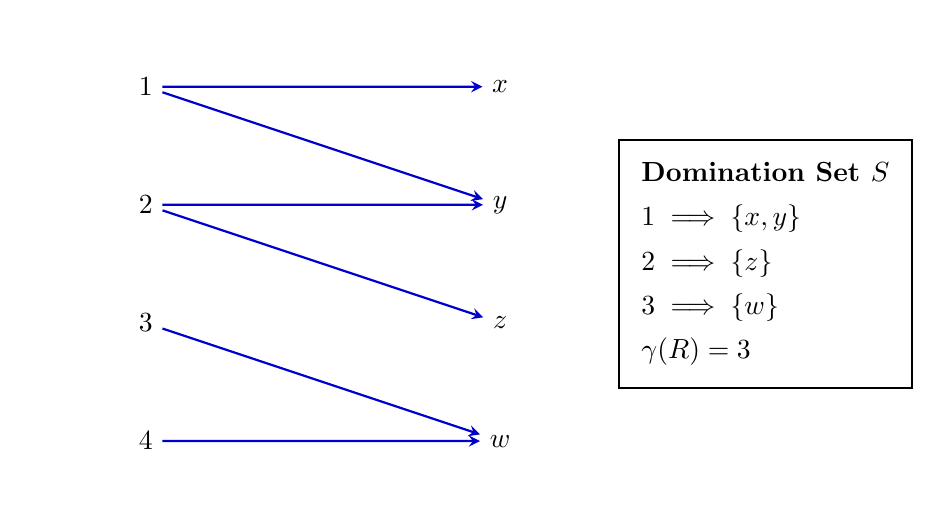
\begin{tikzpicture}[scale=1.5]
    \fill[white] (-1,-1) rectangle (4,3);
    
    % Nodes for A
    \node (a1) at (0, 2.5) {$1$};
    \node (a2) at (0, 1.5) {$2$};
    \node (a3) at (0, 0.5) {$3$};
    \node (a4) at (0, -0.5) {$4$};
    
    % Nodes for B
    \node (b1) at (3, 2.5) {$x$};
    \node (b2) at (3, 1.5) {$y$};
    \node (b3) at (3, 0.5) {$z$};
    \node (b4) at (3, -0.5) {$w$};
    
    % Edges
    \draw[->, >=stealth, thick, blue!80!black] (a1) -- (b1);
    \draw[->, >=stealth, thick, blue!80!black] (a1) -- (b2);
    \draw[->, >=stealth, thick, blue!80!black] (a2) -- (b2);
    \draw[->, >=stealth, thick, blue!80!black] (a2) -- (b3);
    \draw[->, >=stealth, thick, blue!80!black] (a3) -- (b4);
    \draw[->, >=stealth, thick, blue!80!black] (a4) -- (b4);
    
    % Legend
    \node[align=left, inner sep=8pt, anchor=west, draw, thick] at (4, 1) {
        \textbf{Domination Set $S$}\\[4pt]
        $1 \implies \{x, y\}$\\[4pt]
        $2 \implies \{z\}$\\[4pt]
        $3 \implies \{w\}$\\[4pt]
        $\gamma(R) = 3$
    };
\end{tikzpicture}
\end{center}
\end{proof}

\begin{proof}[Solution to Problem 21]
Let $f(x) = x^3 + x$. \\
\textbf{Injectivity:} We use the derivative test. $f'(x) = 3x^2 + 1$. Since $x^2 \ge 0$ for all $x \in \R$, $3x^2 + 1 \ge 1 > 0$. Because the derivative is strictly positive everywhere, $f(x)$ is strictly monotonically increasing. A strictly monotonic function is always injective. \\
\textbf{Surjectivity:} $f(x)$ is a continuous polynomial. As $x \to \infty$, $f(x) \to \infty$. As $x \to -\infty$, $f(x) \to -\infty$. By the Intermediate Value Theorem, $f(x)$ takes on all real values between $-\infty$ and $\infty$. Thus, the range is $\R$, making it surjective. \\
Therefore, $f$ is bijective.
\end{proof}

\begin{proof}[Solution to Problem 22]
Let $f(x) = e^x + x$. \\
\textbf{Injectivity:} $f'(x) = e^x + 1$. Since $e^x > 0$ for all $x \in \R$, $f'(x) > 1 > 0$. The function is strictly increasing, hence injective. \\
\textbf{Surjectivity:} $f(x)$ is continuous. As $x \to \infty$, $e^x \to \infty$ and $x \to \infty$, so $f(x) \to \infty$. As $x \to -\infty$, $e^x \to 0$ and $x \to -\infty$, so $f(x) \to -\infty$. By the Intermediate Value Theorem, the range is $\R$. Thus, $f$ is surjective and therefore bijective.
\end{proof}

\begin{proof}[Solution to Problem 23]
The standard restriction for $f(x) = \sin(x)$ is the domain $[-\pi/2, \pi/2]$ and codomain $[-1, 1]$. \\
\textbf{Injectivity:} On the open interval $(-\pi/2, \pi/2)$, $f'(x) = \cos(x) > 0$. Thus, the function is strictly increasing on the closed interval $[-\pi/2, \pi/2]$, guaranteeing injectivity. \\
\textbf{Surjectivity:} $f(-\pi/2) = -1$ and $f(\pi/2) = 1$. Since $\sin(x)$ is continuous, by the Intermediate Value Theorem, it takes on every value in the interval $[-1, 1]$. Since the codomain is defined as $[-1, 1]$, it is surjective.
\end{proof}

\begin{proof}[Solution to Problem 24]
We must construct an injective function $f : \N \to \Q$. (Assume $\N = \{1, 2, 3, \dots\}$). \\
Define $f(n) = \frac{n}{1} = n$. \\
Let $a, b \in \N$ and assume $f(a) = f(b)$. Then $a = b$. Thus, $f$ is trivially injective. \\
\textit{Remark:} This simple injection proves $|\N| \le |\Q|$. (A bijection requires a much more complex mapping, such as Cantor's pairing function, but the prompt only asked for an injection).
\end{proof}

\begin{proof}[Solution to Problem 25]
To use the Cantor-Schröder-Bernstein Theorem, we need an injection $f : (0, 1) \to [0, 1)$ and an injection $g : [0, 1) \to (0, 1)$. \\
1. Define $f(x) = x$. Since $(0, 1) \subset [0, 1)$, this identity mapping is trivially injective. \\
2. Define $g(x) = \frac{1}{2}x + \frac{1}{4}$. Let $a, b \in [0, 1)$ and assume $g(a) = g(b)$.
\[ \frac{1}{2}a + \frac{1}{4} = \frac{1}{2}b + \frac{1}{4} \implies \frac{1}{2}a = \frac{1}{2}b \implies a = b \]
Thus $g$ is injective. We must verify the range of $g$ is within $(0, 1)$. Since $0 \le x < 1$, we have $0 \le \frac{1}{2}x < \frac{1}{2}$, and thus $\frac{1}{4} \le \frac{1}{2}x + \frac{1}{4} < \frac{3}{4}$. The range is $[1/4, 3/4) \subset (0, 1)$. \\
Since we have injective functions in both directions, by the Cantor-Schröder-Bernstein Theorem, a bijection exists, meaning $|(0, 1)| = |[0, 1)|$.
\end{proof}

\begin{proof}[Solution to Problem 26]
Suppose for contradiction there exists a surjective function $f : A \to \mathcal{P}(A)$. \\
Define a subset $B \subseteq A$ as follows:
\[ B = \{ x \in A \mid x \notin f(x) \} \]
Since $B$ is a subset of $A$, $B \in \mathcal{P}(A)$. Because $f$ is surjective, there must exist some element $a \in A$ such that $f(a) = B$. \\
We now ask: Is $a \in B$? \\
Case 1: Assume $a \in B$. By the definition of $B$, this means $a \notin f(a)$. Since $f(a) = B$, this means $a \notin B$. Contradiction. \\
Case 2: Assume $a \notin B$. Since $f(a) = B$, this means $a \notin f(a)$. By the definition of $B$, any element $x \notin f(x)$ must be in $B$. Thus $a \in B$. Contradiction. \\
Both cases lead to a logical paradox. Therefore, our initial assumption that a surjective function $f$ exists must be false.
\end{proof}

\begin{proof}[Solution to Problem 27]
We are given $Z \sim \mathcal{N}(0, 1)$ with $p_Z(z) = \frac{1}{\sqrt{2\pi}} e^{-z^2/2}$. \\
The transformation is $X = f(Z) = e^Z$. The inverse function is $Z = f^{-1}(X) = \ln(X)$. \\
The derivative of the inverse is $\frac{d}{dx} f^{-1}(x) = \frac{1}{x}$. \\
By the pushforward measure (Change of Variables formula) for a bijective transformation:
\[ p_X(x) = p_Z(f^{-1}(x)) \cdot \left| \frac{d}{dx} f^{-1}(x) \right| \]
Substitute the known functions:
\[ p_X(x) = \frac{1}{\sqrt{2\pi}} \exp\left(-\frac{(\ln x)^2}{2}\right) \cdot \left| \frac{1}{x} \right| \]
Since $X = e^Z > 0$, $|1/x| = 1/x$. Thus, for $x > 0$:
\[ p_X(x) = \frac{1}{x \sqrt{2\pi}} \exp\left(-\frac{(\ln x)^2}{2}\right) \]
This is the exact PDF of the Lognormal distribution.
\end{proof}

\begin{proof}[Solution to Problem 28]
We want to find the distribution of $U = F_X(X)$. We do this by finding its CDF, $F_U(u) = \Prob(U \le u)$. \\
Since $F_X$ is a strictly increasing bijection from $\R$ to $(0, 1)$, its inverse $F_X^{-1}$ exists and is strictly increasing. \\
For $u \in (0, 1)$:
\[ F_U(u) = \Prob(U \le u) = \Prob(F_X(X) \le u) \]
Applying the strictly increasing inverse function $F_X^{-1}$ to both sides of the inequality preserves the inequality direction:
\[ \Prob(X \le F_X^{-1}(u)) \]
By definition, the CDF of $X$ evaluated at $x$ is $\Prob(X \le x)$. Thus:
\[ \Prob(X \le F_X^{-1}(u)) = F_X(F_X^{-1}(u)) = u \]
So $F_U(u) = u$ for $u \in (0, 1)$. This is exactly the CDF of a standard Uniform(0, 1) random variable.
\end{proof}

\begin{proof}[Solution to Problem 29]
Let $f(x, y) = (x + y, x - y)$. Let $u = x + y$ and $v = x - y$. \\
\textbf{Bijectivity:} We solve for $x$ and $y$ in terms of $u$ and $v$. Adding the equations gives $u + v = 2x \implies x = \frac{u+v}{2}$. Subtracting gives $u - v = 2y \implies y = \frac{u-v}{2}$. Since every $(u, v) \in \R^2$ yields a unique $(x, y) \in \R^2$, the function has a well-defined two-sided inverse, making it bijective. \\
\textbf{Jacobian Determinant:} The Jacobian matrix $J$ is:
\[ J = \begin{pmatrix} \frac{\partial u}{\partial x} & \frac{\partial u}{\partial y} \\ \frac{\partial v}{\partial x} & \frac{\partial v}{\partial y} \end{pmatrix} = \begin{pmatrix} 1 & 1 \\ 1 & -1 \end{pmatrix} \]
\[ \det(J) = (1)(-1) - (1)(1) = -1 - 1 = -2 \]
\textbf{Explanation:} In probability transformations (like Normalizing Flows), the absolute value of the Jacobian determinant $|\det(J)|$ represents the local scaling factor of the volume space. If $\det(J) = 0$, the space collapses into a lower dimension, destroying bijectivity and causing the probability density to become undefined (division by zero in the pushforward measure).
\end{proof}

\begin{proof}[Solution to Problem 30]
\textbf{The Flaw:} The proof falsely applies Theorem 1.2 (Finiteness and Bijections) to an infinite set. \\
Theorem 1.2 explicitly states: "Let $A$ and $B$ be \textbf{finite} nonempty sets such that $|A| = |B|$... then $f$ is injective if and only if $f$ is surjective." \\
The set of integers $\Z$ is an infinite set. For infinite sets, injectivity does \textit{not} guarantee surjectivity, even if the domain and codomain are the same set. \\
\textbf{Counterexample to Surjectivity:} Let $y = 3 \in \Z$. We require $4n = 3 \implies n = 3/4$. Since $3/4 \notin \Z$, the element 3 has no pre-image. Thus, $f(n) = 4n$ is strictly injective but not surjective.
\end{proof}

\newpage

\section{Concept Checklist \& Question Mapping (Repeated)}
\label{sec:concept_checklist_end}

\renewcommand{\arraystretch}{1.5}
\begin{tabularx}{\textwidth}{>{\bfseries}l X >{$\displaystyle}c<{$}}
\toprule
\textbf{ID} & \textbf{Concept / Proof Technique} & \text{\textbf{Problems}} \\
\midrule
C1 & Algebraic Bijections (Linear, Quadratic, Rational) & 1, 2, 3, 4, 5 \\
C2 & Modular Arithmetic \& Equivalence Classes ($\Z_n$) & 6, 7, 8 \\
C3 & Set-Theoretic Proofs (Images, Pre-images, Subsets) & 9, 10, 11, 12 \\
C4 & Function Composition \& Left/Right Inverses & 13, 14, 15, 16 \\
C5 & Combinatorics, Pigeonhole, \& Hall's Marriage & 17, 18, 19, 20 \\
C6 & Calculus-Based Bijections (Derivatives, IVT) & 21, 22, 23 \\
C7 & Infinite Sets \& Cantor-Schröder-Bernstein Theorem & 24, 25, 26 \\
C8 & Real-World Modeling: Normalizing Flows \& Copulas & 27, 28, 29 \\
C9 & Logical Fallacies \& Axiomatic Edge Cases & 30 \\
\bottomrule
\end{tabularx}

\end{document}